Diabetes mellitus je metabolická disfunkcia charakterizovaná hyperglykémiou, ktorá je dôsledkom porúch sekrécie inzulínu z pankreasu, účinku inzulínu alebo spojením oboch porúch.\cite{2004}
Chronická hyperglykémia diabetu je spojená s dlhodobým poškodením, dysfunkciou a zlyhaním rôznych orgánov, najmä očí, obličiek, nervov, srdca a ciev.

\begin{figure}[h]
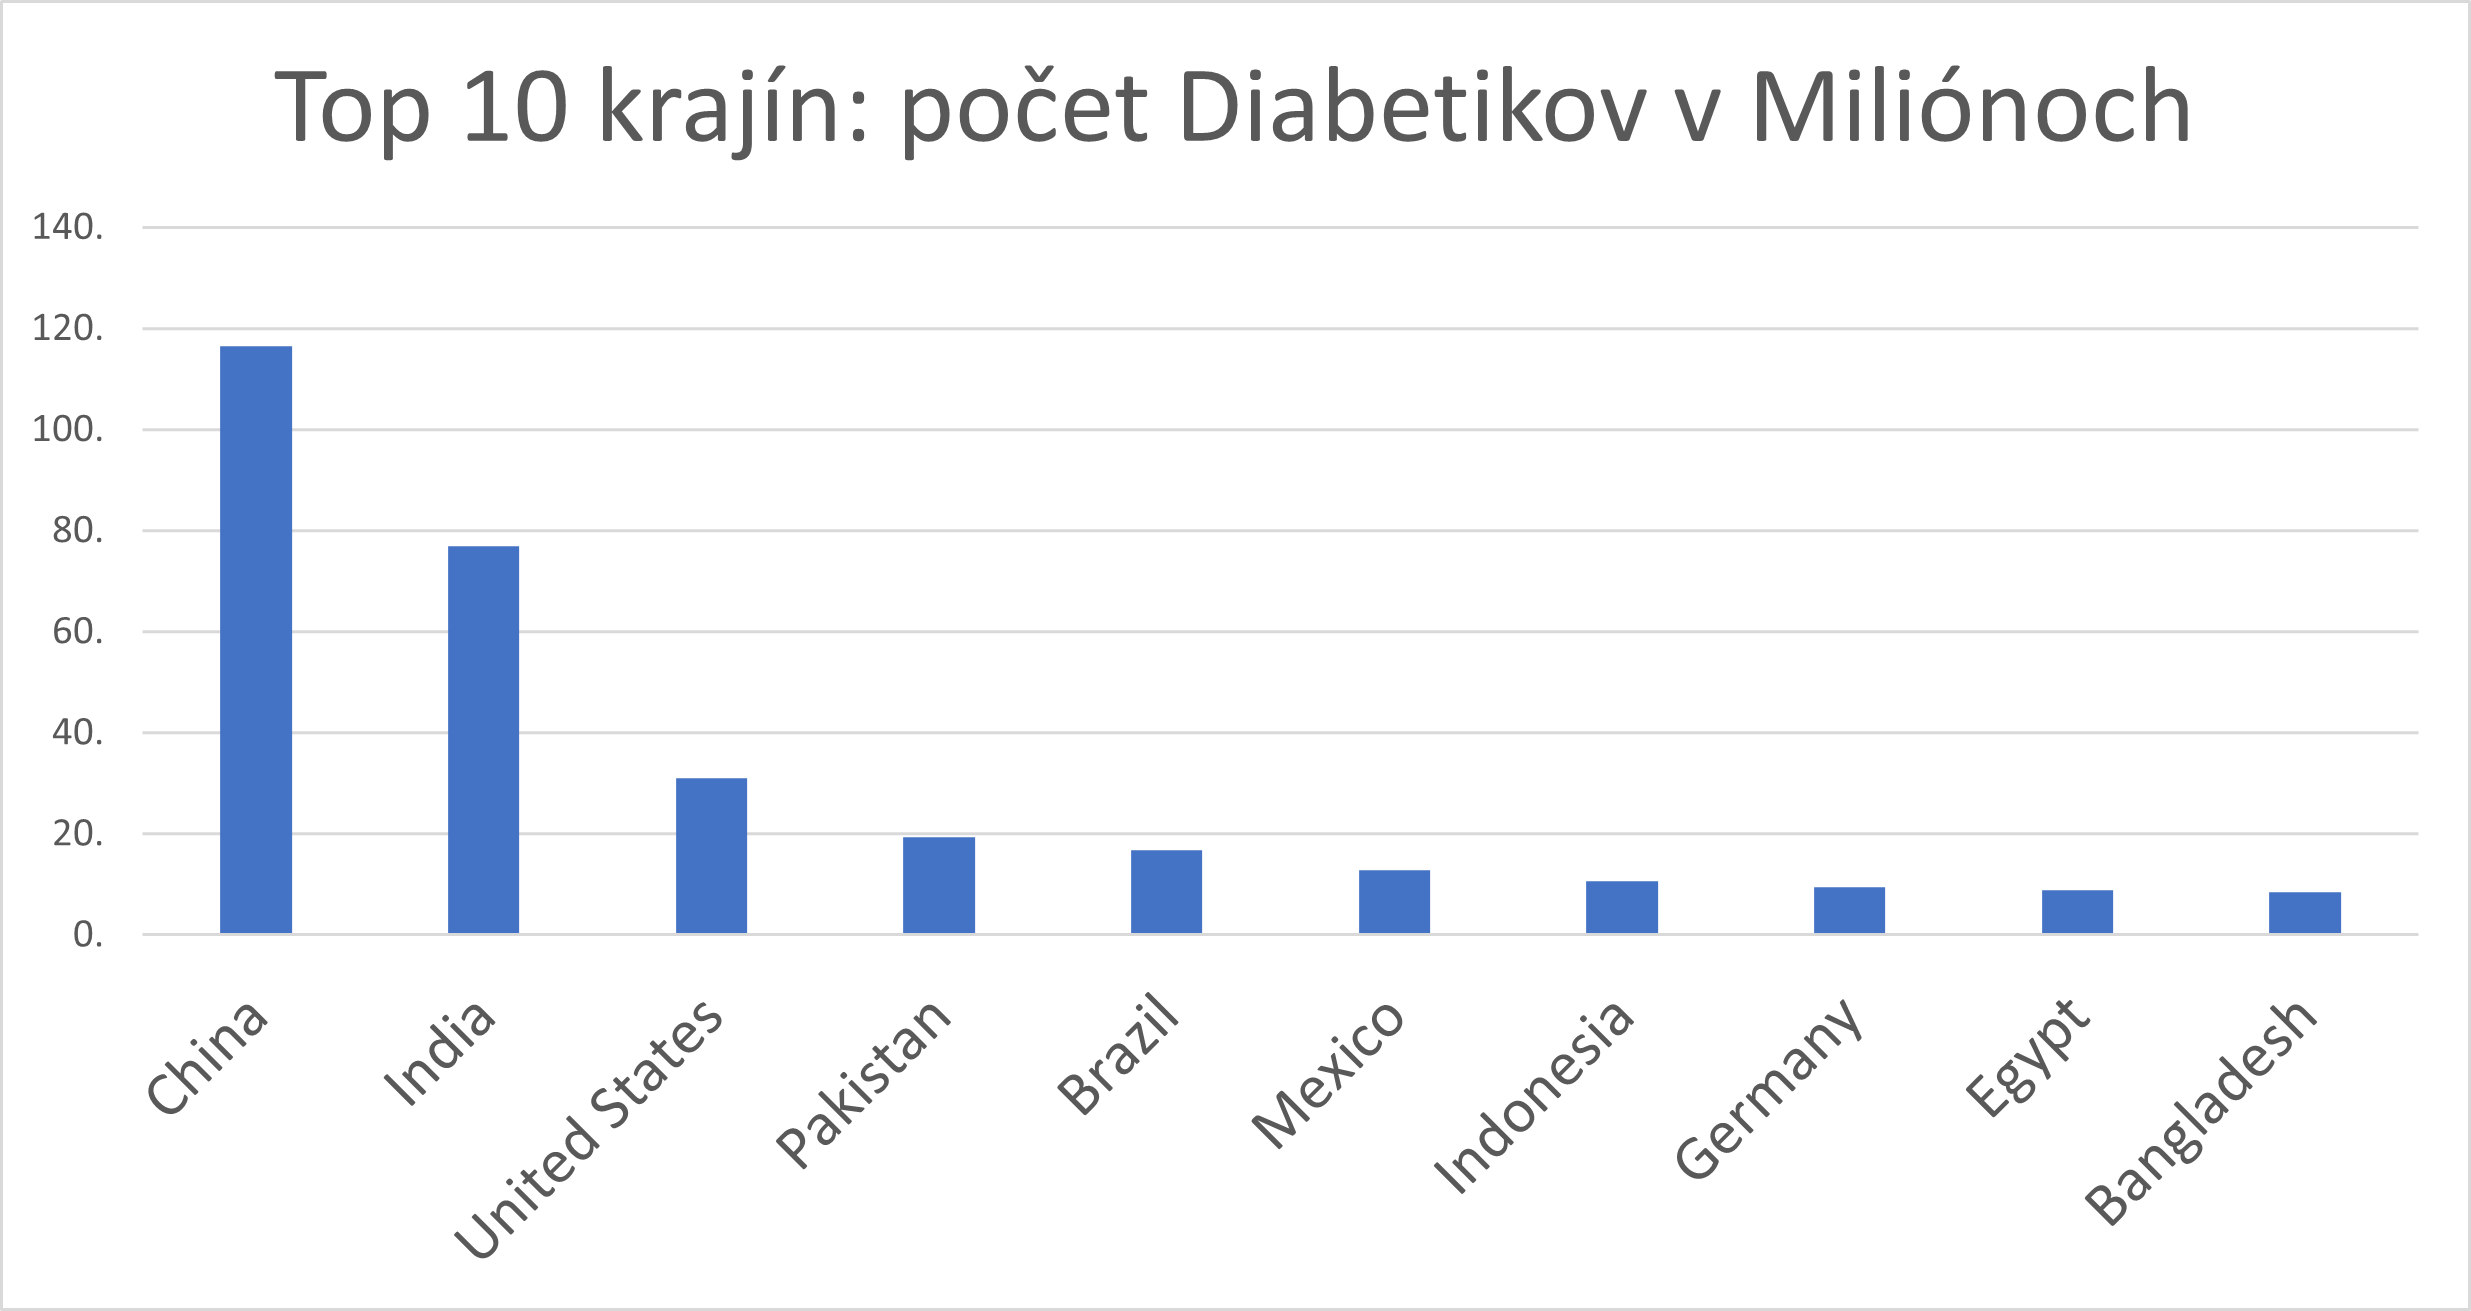
\includegraphics[scale=0.8]{pocet_diabetikov.png}
\caption{graf znázorňujúci počet diabetikov na 1000 obyvateľov podľa pohlavia od 1980 do 2017 \cite{2018}}
\end{figure}

Na vzniku cukrovky sa podieľa niekoľko faktorov. Tieto sa pohybujú od autoimunitnej deštrukcie beta buniek pankreasu s následným nedostatkom inzulínu po abnormality, ktoré vedú k rezistenci bunieki na pôsobenie inzulínu.
Základom abnormalít v metabolizme uhľohydrátov, tukov a bielkovín pri cukrovke je nedostatočné pôsobenie inzulínu na cieľové tkanivá. Nedostatočný účinok inzulínu je dôsledkom nedostatočnej sekrécie inzulínu a/alebo zníženej reakcie tkaniva na inzulín v jednom alebo viacerých bodoch komplexných dráh pôsobenia hormónov. Porušenie sekrécie inzulínu a defekty v pôsobení inzulínu často koexistujú u rovnakého pacienta a často nie je jasné, ktorá abnormalita, či už samotná, je primárnou príčinou hyperglykémie, prípadnej hypoglykémie.\cite{2004}

Medzi príznaky diabetesu patrí strata hmotnosti, alebo obezita, nadmerné močenie, smäd, hlad. Vážnejšími príznakmi sú napríklad zhoršenie zraku, problémy pri močené a iné.
K dlhodobým komplikáciám diabetu patrí retinopatia s potenciálnou stratou zraku; nefropatia vedúca k zlyhaniu obličiek; periférna neuropatia s rizikom vredov na nohách, amputácií a Charcotových kĺbov; a autonómna neuropatia spôsobujúca gastrointestinálne, genitourinárne a kardiovaskulárne symptómy a sexuálnu dysfunkciu. U pacientov s diabetom je zvýšený výskyt aterosklerotických kardiovaskulárnych, periférnych arteriálnych a cerebrovaskulárnych chorôb.\cite{2004}

Prevažná väčšina prípadov cukrovky spadá do dvoch širokých etiopatogenetických kategórií. Pri cukrovke 1. typu, je príčinou absolútny nedostatok sekrécie inzulínu. Jedinci so zvýšeným rizikom vzniku tohto typu diabetu môžu byť často identifikovaní sérologickými dôkazmi autoimunitného patologického procesu vyskytujúceho sa na ostrovčekoch pankreasu. Pri druhej, oveľa rozšírenejšej kategórii, cukrovke typu 2, je príčinou kombinácia odolnosti voči účinku inzulínu a neadekvátnej kompenzačnej sekrečnej reakcie na inzulín. V druhej kategórii môže stupeň hyperglykémie postačujúci na to, aby spôsobil patologické a funkčné zmeny v rôznych cieľových tkanivách, ale bez klinických symptómov, môže jedinec existovať dlhší čas, než sa zistí diabetes. Počas tohto asymptomatického obdobia je možné demonštrovať odchýlku v metabolizme uhľohydrátov meraním plazmatickej glukózy nalačno.\cite{2004}


